% ***********************************************************************************************
%
%																								Results
%
\section{Results}\label{results}
% ***********************************************************************************************
Each section introduced into some theoretical part to guide the reader through our possible approach of how a humanoid robot can autonomously localize in real-time its own hand and afterward detect its hand and why it is important to have such an algorithm. In this section we first name the experimental circumstances and then evaluate the the localization and the detection of the hand of the proposed method with the aid of the \textit{online} results and their \textit{offline} generated co-results of the same sequences.
%
%In each chapter we introduced some theoretical part to guide the reader through our possible approach of how a robot is able to autonomously localize and detect its hand and why it is so important to have such an algorithm. G. Metta et al.\ \cite{PRTL07-01} assume to have a/some visual model of the hand in order to be able to perform a visual guided reaching for grasping an object. Using visual servoing methods, where the arm speed is controlled based upon visual information and lead to a target object, requires the ability to measure the distance between hand and object. If such a visual model is available, reaching can be performed by a coarse approximative approach to the object using open-loop reaching and then perform the positioning for grasping by a closed-loop method. In the evaluation part we will first name the experimental circumstances, followed by the evaluation of the ``live'' results and the artificially gained co-results for equivalent test sets, but with different parameters.

% -----------------------------------------------------------------------------------------------
%
%																						test environment
%
\subsection{Test environment}\label{results:testenv}
% -----------------------------------------------------------------------------------------------
For the online tests James that was moving its arm in front of its face for a certain period of time. 
%
% -----------------------------------------------------------------------------------------------
%
%																	motor sensory stimulation / effection
%
\subsubsection{Motor sensory stimulation/effection}\label{results:motosensstim}
% -----------------------------------------------------------------------------------------------

% -----------------------------------------------------------------------------------------------
%
%																								evaluation
%
\subsection{Evaluation}\label{results:evaluation}
% -----------------------------------------------------------------------------------------------
Besides the original online test results, co-results had to be gained by re-executing the same tests offline from files without using the robot, but with different parameters. During the online tests running on the robot we recorded the original sequences and stored all visual and proprioceptive information. To guarantee a precise and sound evaluation exactly the same information had to be used on whose the method was applied again but only changing the correlation coefficient. Starting from these 10 online test runs we actually gained 100 results. The parameter of interest, the key parameter of this whole approach of finding the hand, is the correlation coefficient that matches trajectories from the different proprioception. Accuracy of our results can only be as good as the correlation threshold. All visual information with motor sensory information, or vice versa, correlate in some amount. So in the end the choice of the threshold defines the quality of the result. A threshold that accepts a low correlation coefficient from a visual and the motor trajectory, that in fact describes dissimilar behaviour, can not result in good localization. On the other hand, correlation can also be chosen too tight, with the effect that we really determine several exact positions of the hand, but unfortunately also skip too many patches that actually belong to the positive set as well, see figure \ref{fig:impactofcorr}. After all, correlation must be determined as a compromise between the well-known trade-offs accuracy and reliability.
%
\begin{figure}
	\begin{center}
		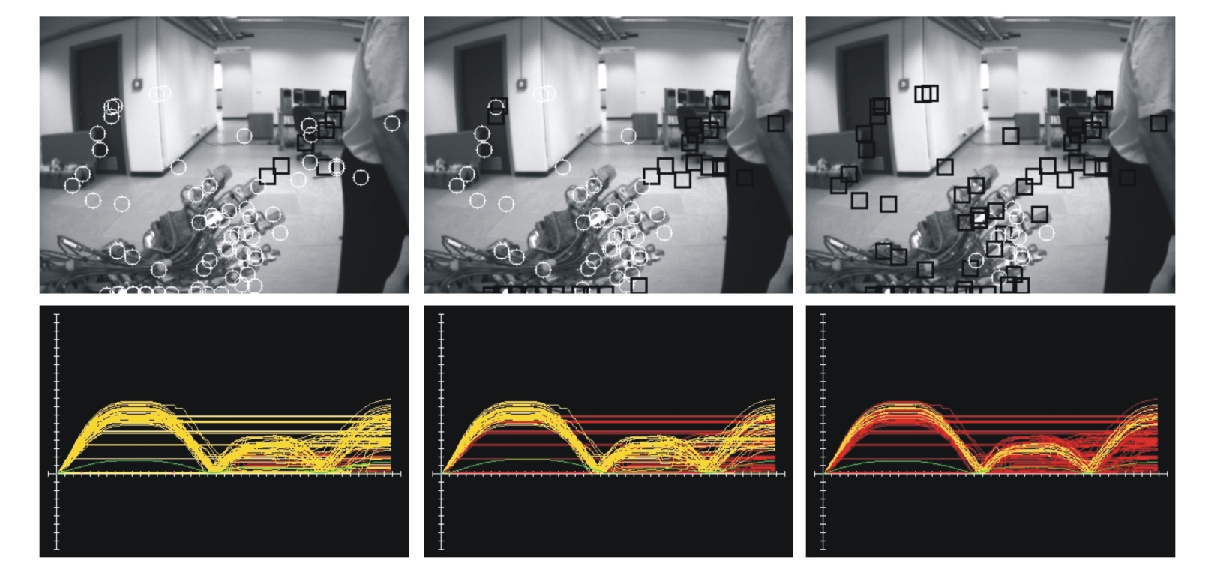
\includegraphics[width=3.5in]{imgs/results/impactofcorr.pdf}
			\caption[Varying the correlation threshold.]{ This figure is illustrating how the correlation has an impact on the number of the correlating patches. From left to right: correlation 0.0, 0.6 and 0.94. }
			\label{fig:impactofcorr}
	\end{center}
\end{figure}
%
\subsubsection{Localization}
\label{results:evaluation:localization}
%
A possible way to rate the outcome of the hand localization process is to transform the visual results into a set of sound numbers. As correlation is the key factor for the accuracy of mapping causal action with motion perception, different outcomes of the same data sets are expected when changing the correlation threshold. Obviously different outcomes by varying the parameter do not mean different locations, but choosing a smaller or larger set of patches that define the region where the hand is located in the visive field. An overview of the results in form of numbers gives table \ref{tab:resultstatitistics}, where the entries were obtained by analyzing the recorded tracking sequences or from the robot's (or module's) output. 
%
The optimal solution had been achieved by manual evaluation of the tracking process and is therefore an absolute and convincing (expressive) measure, with which the automatic choice can be confronted. 

Depending on the correlation threshold patches can be chosen that do actually not belong to the hand. By increasing the correlation coefficient threshold the number of false-positives diminishes rapidly. In the middle graph the false-positive rate is much smaller, but of course also the true-positive rate diminishes. At a correlation threshold of 0.97 a really good classification can be achieved. In some cases, see in the bottom graph test sets 1 and 8-10, the exploitation of patches lying on the hand is very small, but we prefer a small set of patches that really lie on the hand, rather than having false positives. Figure \ref{fig:result:diag} shows the same 10 test series in a different diagram, where the true positive rate (black) and the false positive rate (white) are directly comparable in the bar graphs. FPR is in all cases really small and almost negligible. Test set 9 for instance could be a neglected one if we were applying the algorithm many times in a learning algorithm, on the other hand we can also see that the FPR diminishes by around 50\% when increasing the correlation coefficient. Using this diagram we can see, that raising the correlation threshold from 0.91 to 0.97 doubles the number of test sets without FPs. 

%
\begin{figure}
	\begin{center}
		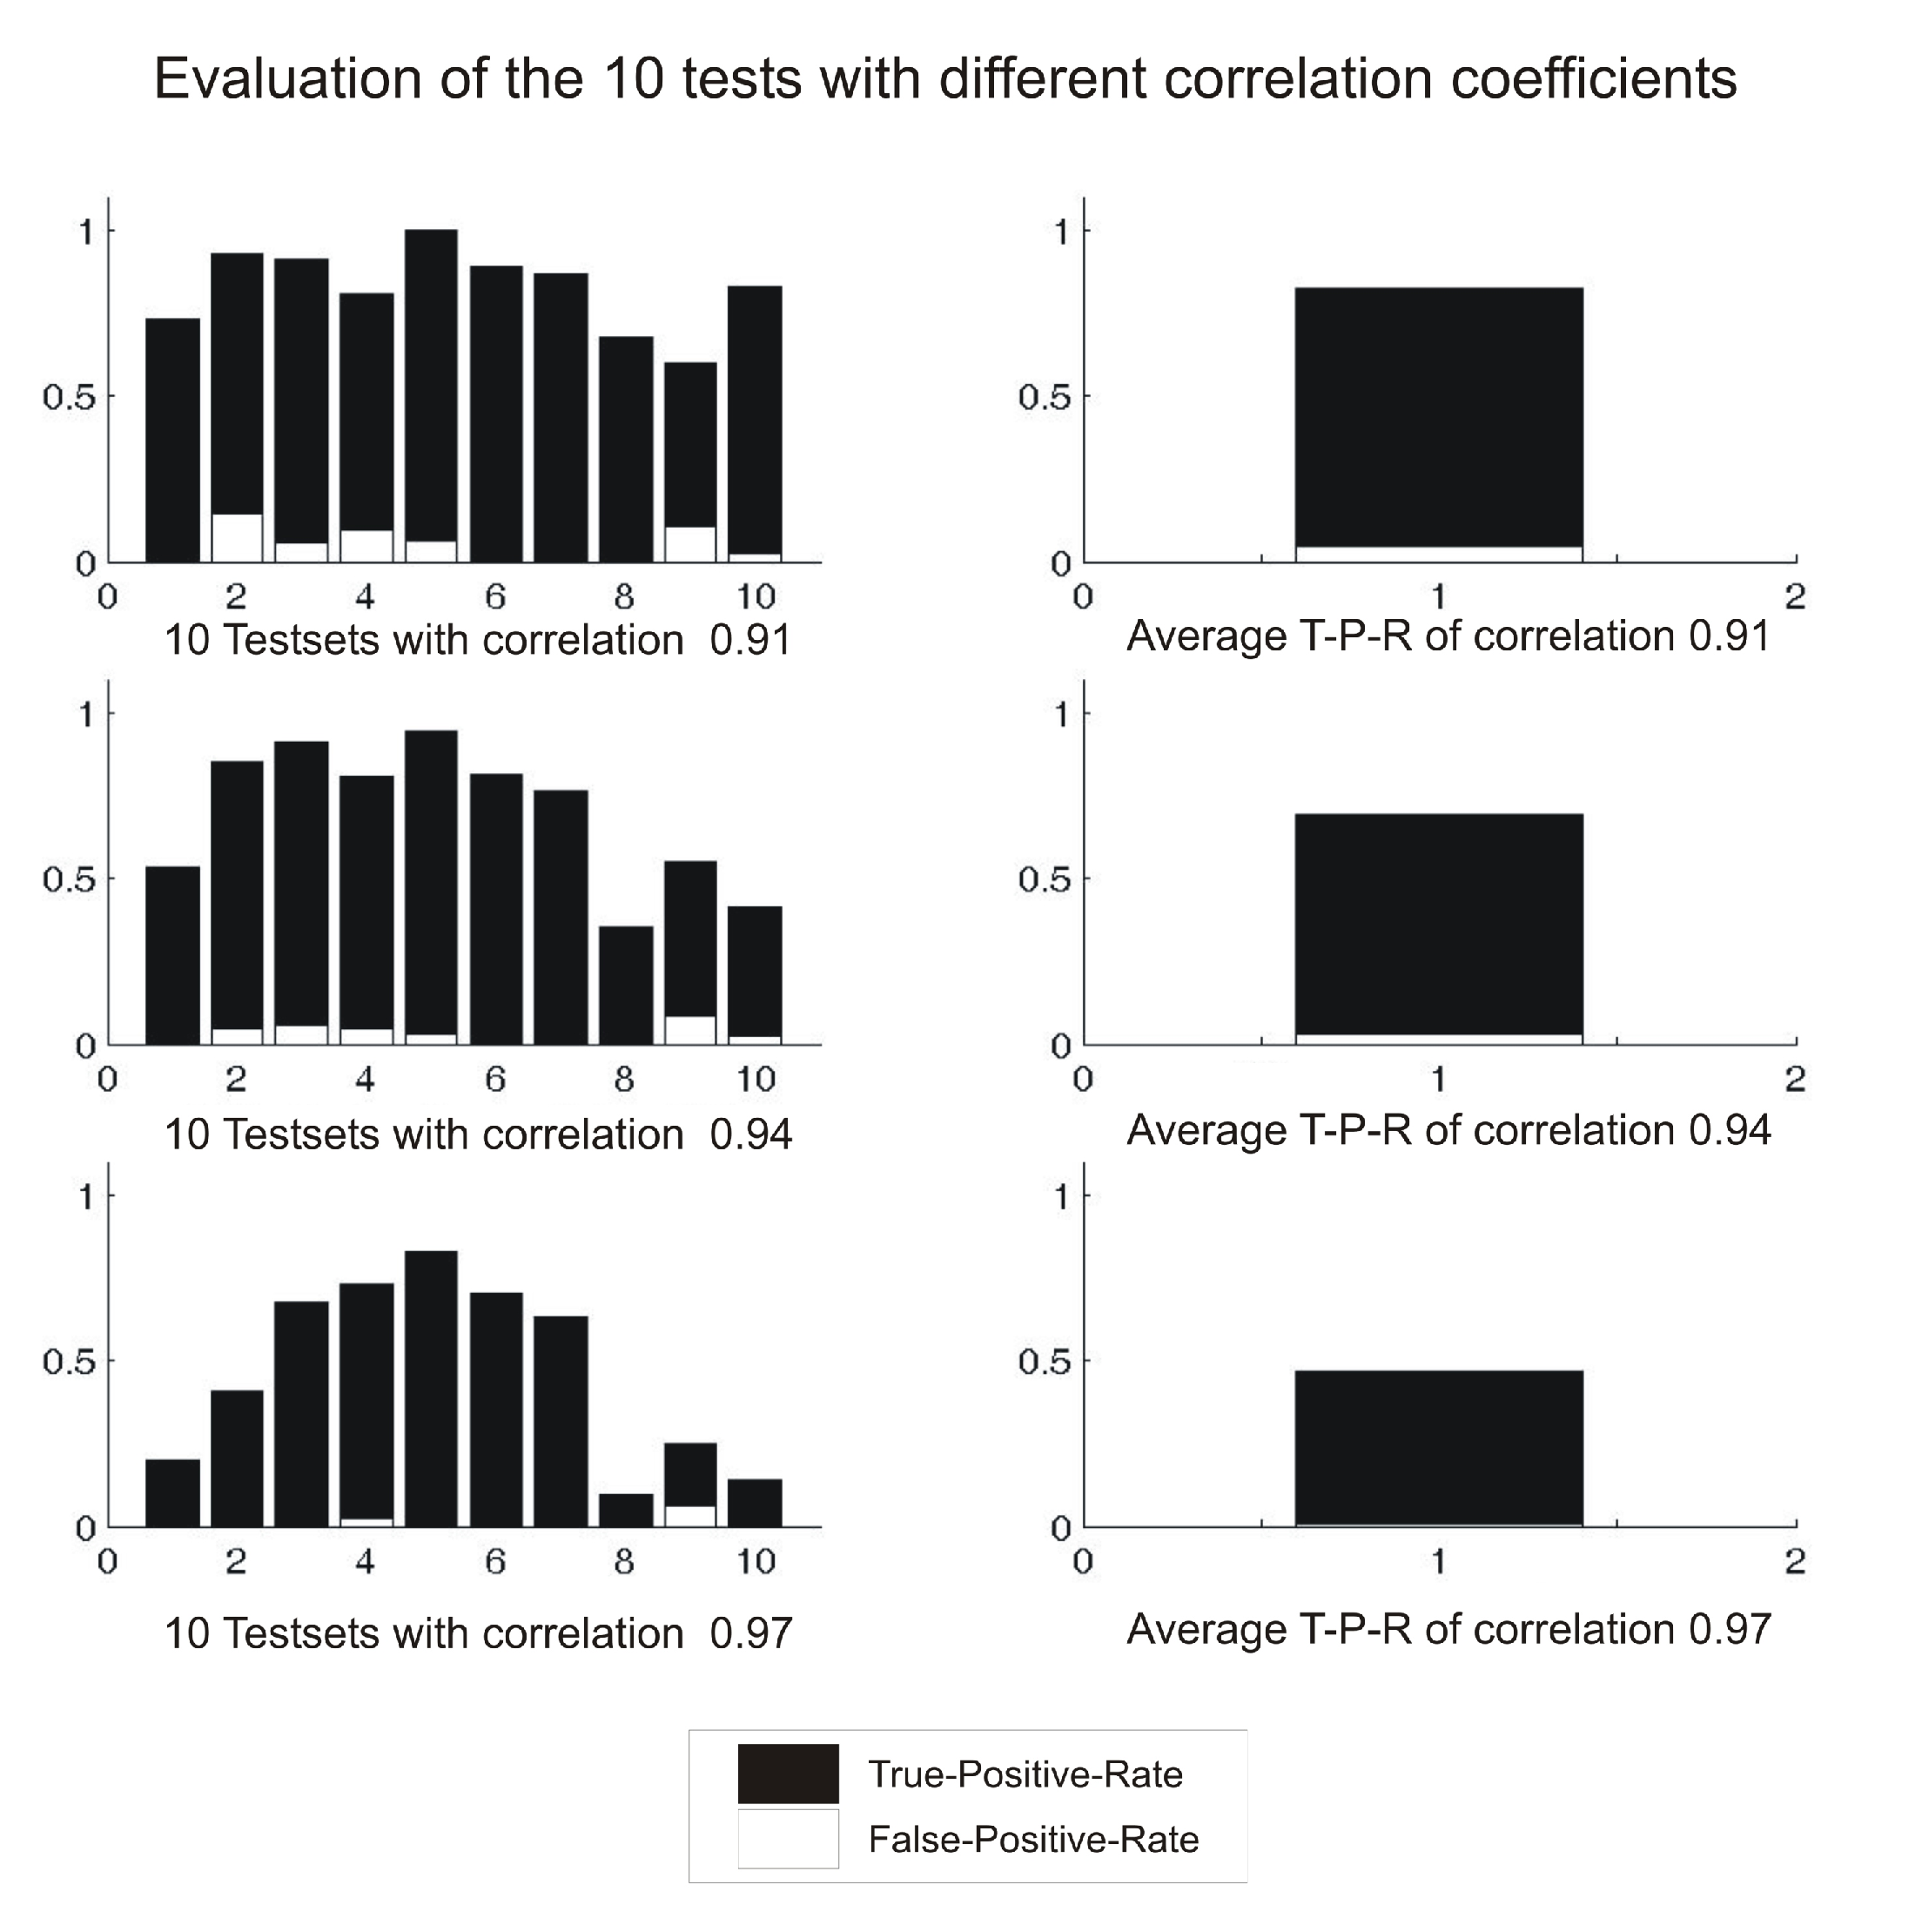
\includegraphics[width=3.5in]{imgs/results/diag.pdf}
			\caption[True and false positive rates of the 10 main test sets. ]{True and false positive rates of the 10 main test sets. The 10 test sets are displayed again with different correlation coefficient thresholds. The average ``learning'' over 10 sets show high reliability and very few FPs. Increasing the threshold from 0.91 to 0.97 effects an increase of the number of test sets without FP from four to 8 test sets.}
			\label{fig:result:diag}
	\end{center}
\end{figure}
%
%
An expressive judgment on the proposed method to localize the hand can be gained with the confrontation of the \textit{False-Positive-Ratio} against the \textit{True-Positive-Ratio} in order to rate our classification algorithm. For a two-class prediction system a graphical plot for visualizing performance and organizing classifiers, here the correlation coefficient, the Receiver-Operating-Characteristics (ROC) graphs plot the sensitivity versus (1-specificity) \cite{ROC04-03}. The entire set of outcomes are either marked as \textbf{P}ositives, which denote all correct solutions of patches that were following the hand, or \textbf{N}egatives, that are the whole set without the positive ones from all tracked patches. %A prediction can be falsely classified as a positive when it is actually negative, this false-alarm is called a \textbf{F}alse-\textbf{P}ositive. 
For a \textbf{T}rue-\textbf{P}ositive the actual and the prediction values are both positives, in our case TP determine the number of ``hand classified'' patches that have really been on the hand. %To build the ROC curve, only the FPR and the TPR are needed. 
The TPR, the sensitivity, determines how many positive instances have been correctly classified as positives among all positives available at one test. The ratio of costly false-positives among all negatives define the false-alarm rate, FPR, and is equal to 1-specificity. %A perfect classification would have hundred per cent specificity, no FP, and hundred per cent sensitivity, where all true positives are found, and would get the coordinate (0;1) in the ROC space. 
The ROC space illustrates the trade-off between true (y-axis) and false positives (x-axis). In order to get an expressive ROC the online tests have been reproduced offline for the correlation thresholds 0.0, 0.1, 0.2, ..., 0.9, 0.91, 0.97 and 1.0. In order to classify the patches behaviour and decide on the correctness of the methods output all the sequences had to be elaborated by hand. The outcome of the hand localization shows an extremely good ROC far away from any random classification and confirms the resulting ROIs, see examples in figure \ref{fig:roi}. Even under difficult and noisy circumstances it shows good results.
%
\begin{figure}
	\begin{center}
		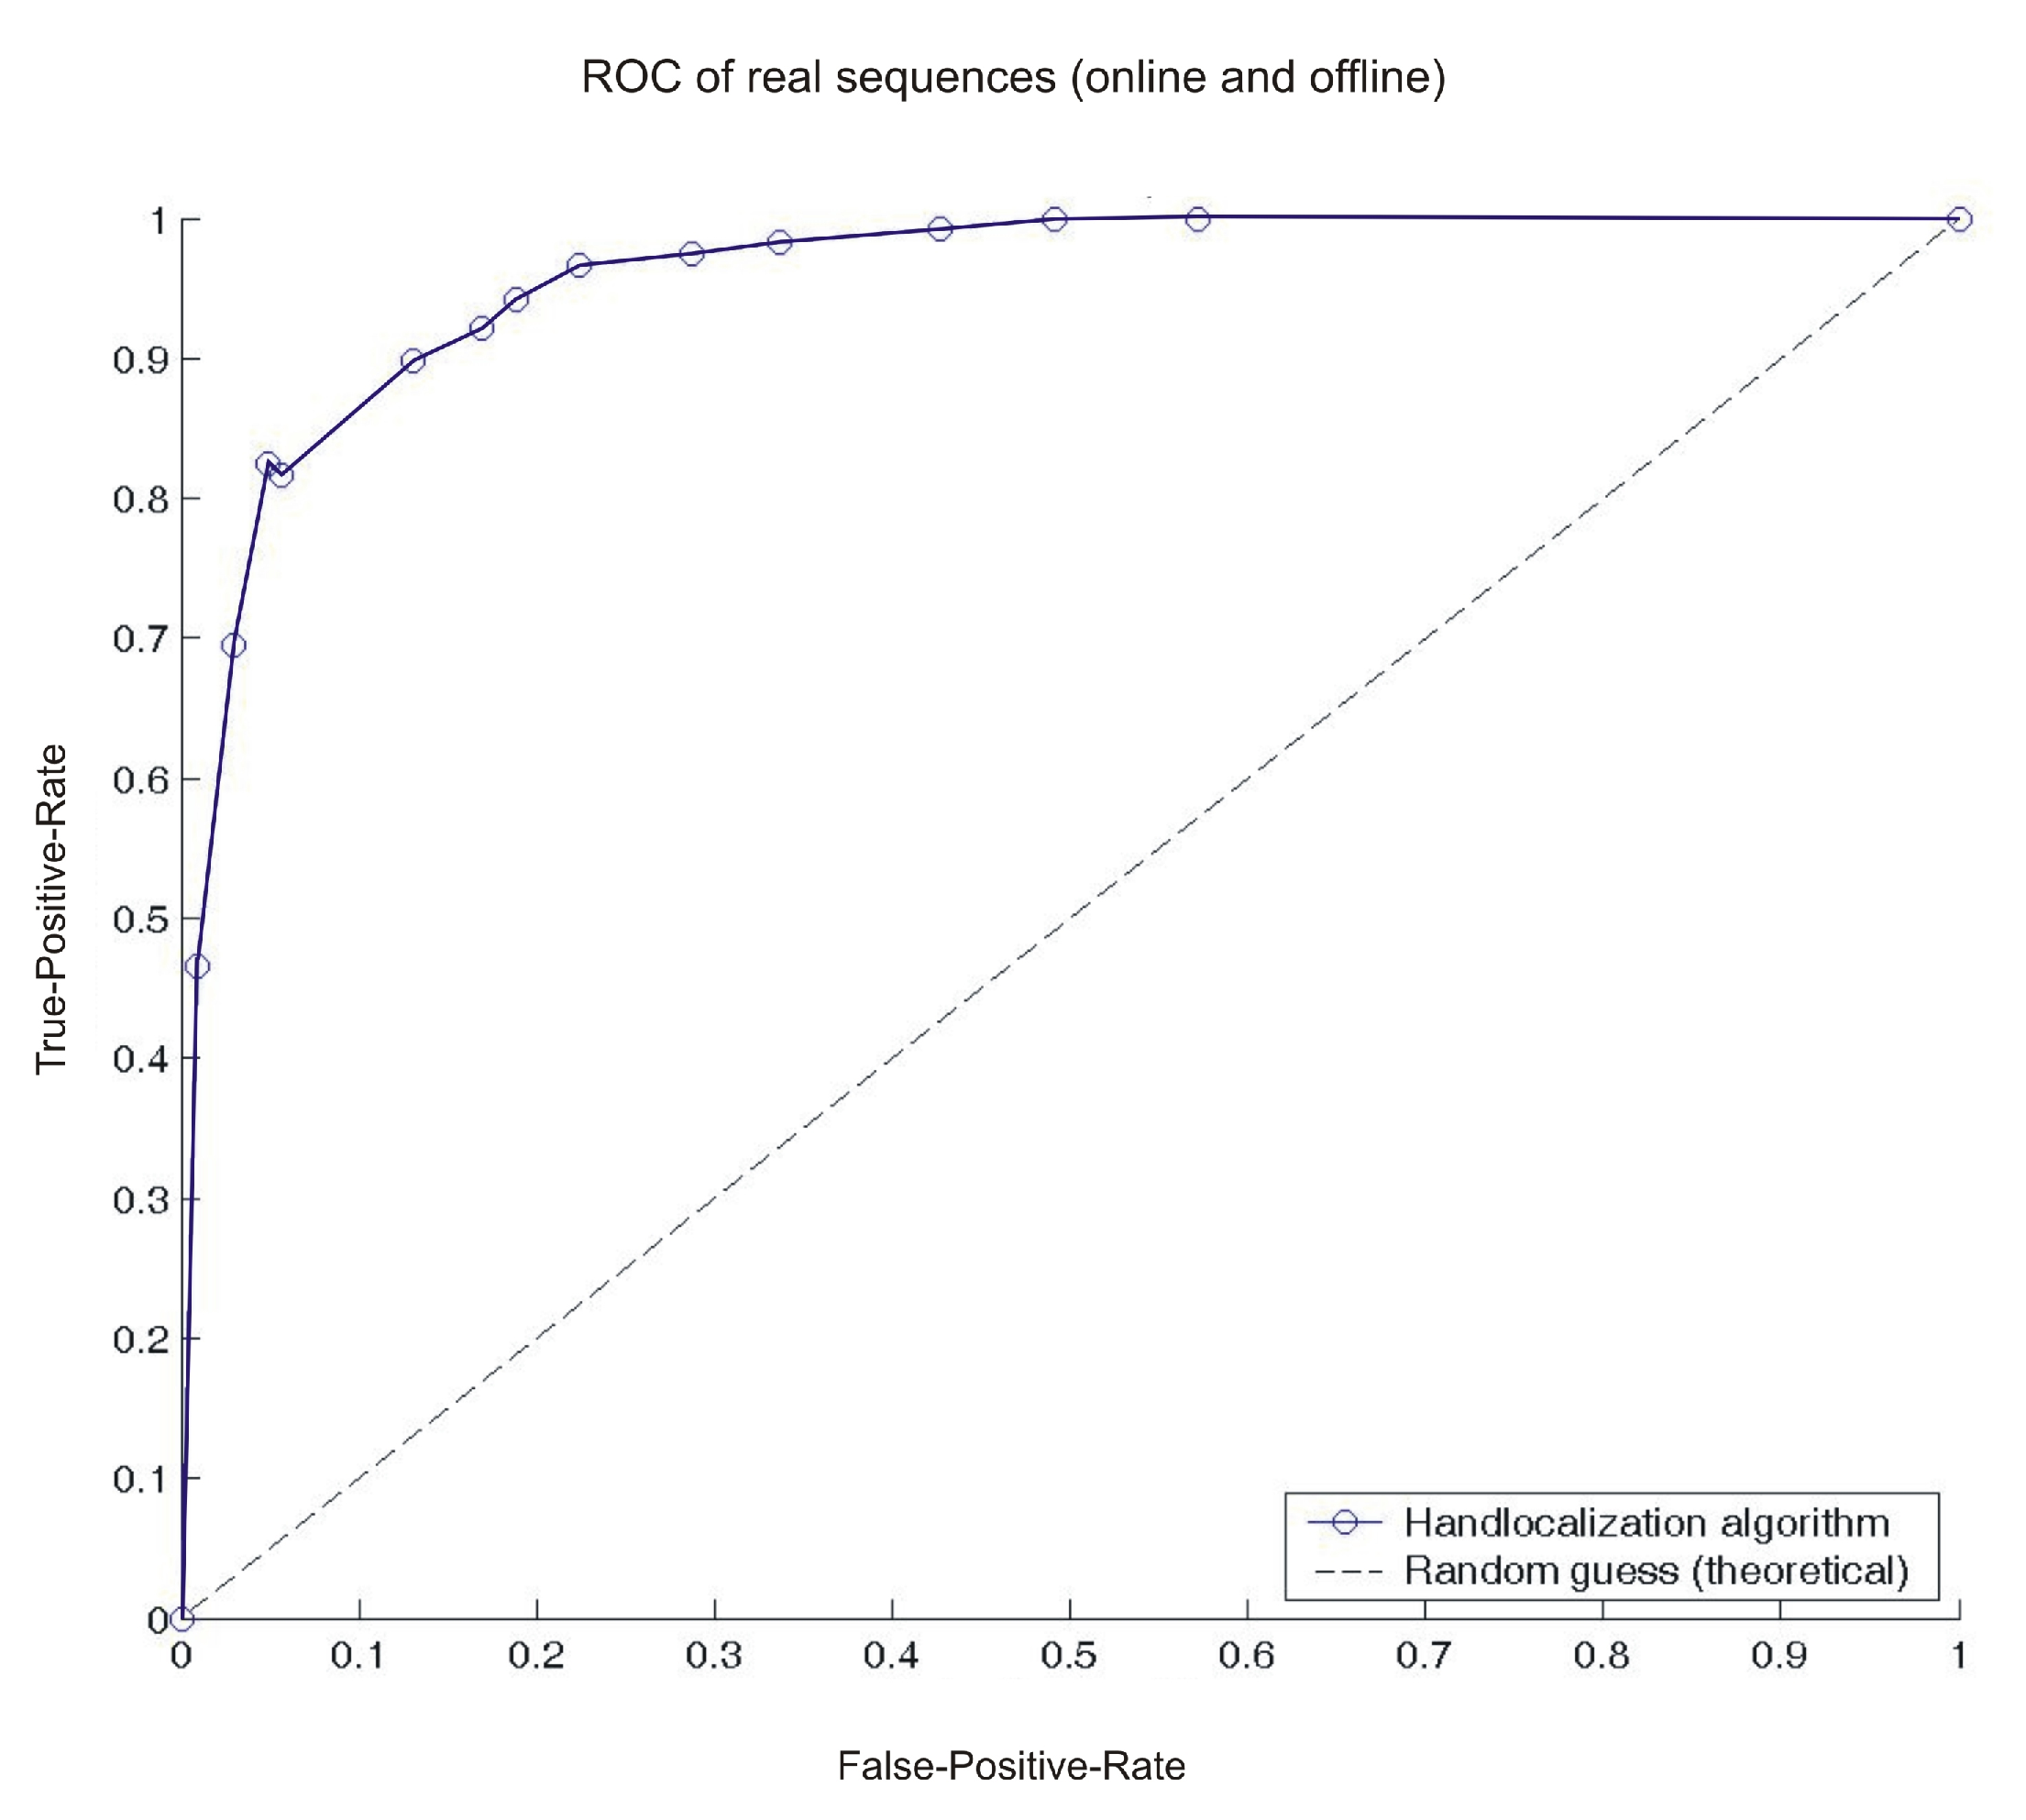
\includegraphics[width=3.5in]{imgs/results/roc.pdf}
			\caption[Receiver-Operating-Characteristics graph for the 10 main test sets. ]{Receiver-Operating-Characteristics graph for the 10 main test sets. The ROC has been created with the 10 raw data sets of the online tests and correlation from 0.0 to 1.0. Our ROC is nearly perfect. As a consequence, this objective ROC testimonies us an algorithm that is highly reliable finding the correct patches of the hand and this under different circumstances and environments. Already from very low correlation coefficients we can see that FPs are below 0.5. }
			\label{fig:result:roc}
	\end{center}
\end{figure}
%
%
\subsubsection{Detection (Segmentation)}
\label{results:evaluation:segmentation}
%
The segmentation process' result is simple to rate. By subtracting the background from the image where the hand had been localized, the foreground is recovered. A good result is achieved, if the foreground exactly depicts the hand. Having the background perfectly recovered with the method after A.Colombari et al \cite{} Completeness of the background initialization method depends a lot on choosing the correct amount of pictures and on the heuristic assumptions proposed in \cite{BICS06}. During tests and implementation we found out that a few constraints of the BICS algorithm are very strict and therefore can cause undesired results in a every day use of the algorithm in a robot where the hand for instance will not release all the background. The method is also too vulnerable if not at least two patches from the correspondent temporal footprint have seen entirely the background. Already a small entity, that differs in a patch from the real background, causes a large distance measure with the consequence to be excluded. One might think that in a sequence of 200 images it must be possible that each patch was fully revealed at least twice. Unfortunately under daily circumstances this constraint is not the case, as our experiments showed us. Embedding our entire algorithm in a learning mechanism could only partly solve the problem. During the evaluation we found out that it would actually make sense to selectively pick images with ``good'' properties for the BICS-algorithm. Images that are anyway present, and information about trajectories can help a lot in selecting images for a reliable, effective and efficient background retrieval. As an example, images could be chosen where the hand was not present in the ROI, what we can roughly assume by evaluating the trajectories of the ``robot''-patches. 